The proposed system is implemented and evaluated using the 1920 RGB images described in section \ref{daq}. The first result that is evaluated is the effect of PCA on the accuracy of the classifier. We use 5-fold cross validation on a bagged decision tree ensemble with 25 trees as a starting point. This is used to compare the accuracies of using the unreduced input, PCA reduction to maintain 99\% variance and PCA reduction to maintain 95\% variance. As shown in Table \ref{tab:pca_comp}, the drop in accuracy is over 10\%, which is not acceptable for an application of this nature. Therefore, from this point on, no PCA is used.

\bgroup
\def\arraystretch{1.5}
\begin{table}[htbp]
	\caption{5-Fold Cross Validation Accuracies of Various PCA Levels}
	\begin{center}
		\begin{tabular}{|l|>{\centering\arraybackslash}m{1.75cm}|>{\centering\arraybackslash}m{1.75cm}|>{\centering\arraybackslash}m{1.75cm}|}
			\hline
			& \textbf{No PCA} & \textbf{99\% Variance PCA} & \textbf{95\% Variance PCA} \\
			\hline
			\# \textbf{Components} & 12596 & 1234 & 700 \\
			\hline
			\textbf{Accuracy} & 99.0625\% & 87.2917\% & 89.4792\% \\
			\hline
		\end{tabular}
		\label{tab:pca_comp}
	\end{center}
\end{table}
\egroup

The objective is to reduce computational complexity and get a good runtime. Thus, more trees than necessary should not be used in the ensemble classifier. To find the optimal number of trees, we perform 5-fold cross validation while varying the number of trees. From the result, shown in Fig. \ref{fig:num_trees}, some fluctuation in accuracy is shown when increasing the tree count past 7. However, this is likely due to the data being split up randomly when performing 5-fold cross validation. Therefore, it is safe to assume that the accuracy is fairly constant past 5 trees. This leads us to select 5 trees as the optimal number of trees.

\begin{figure}[tp]
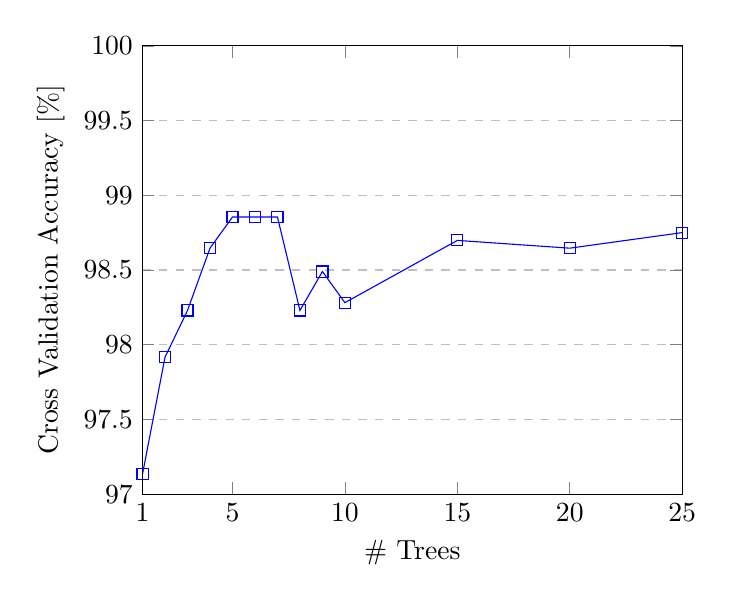
\begin{tikzpicture}
\begin{axis}[
xlabel={\# Trees},
ylabel={Cross Validation Accuracy [\%]},
xmin=1, xmax=25,
ymin=97, ymax=100,
xtick={1,5,10,15,20,25},
ytick={97.0,97.5,98.0,98.5,99.0,99.5,100.0},
ymajorgrids=true,
grid style=dashed,
]

\addplot[
color=blue,
mark=square,
]
coordinates {
	(1,97.1354)(2,97.9167)(3,98.2292)(4,98.6458)(5,98.8542)(6,98.8542)(7,98.8542)(8,98.2292)(9,98.4896)(10,98.2812)(15,98.6979)(20,98.6458)(25,98.75)
};

\end{axis}
\end{tikzpicture}
\caption{The effect of the number of trees on 5-fold cross validation accuracy.}
\label{fig:num_trees}
\end{figure}

To verify that this is indeed a good model all-round and is tolerant to different data-sizes, we perform k-fold cross validation varying k. The result, shown in Fig. \ref{fig:k_fold}, confirms the constancy of the classifier. Finally, we compare the accuracy and runtime of our classifier with Inception (see Table \ref{tab:inception_comp}), an established and successful DNN \cite{b6_1}. While the accuracy of our classifier is slighly lower than that of Inception, its runtime is significantly faster, proving to be a viable alternative.

\begin{figure}[tp]
	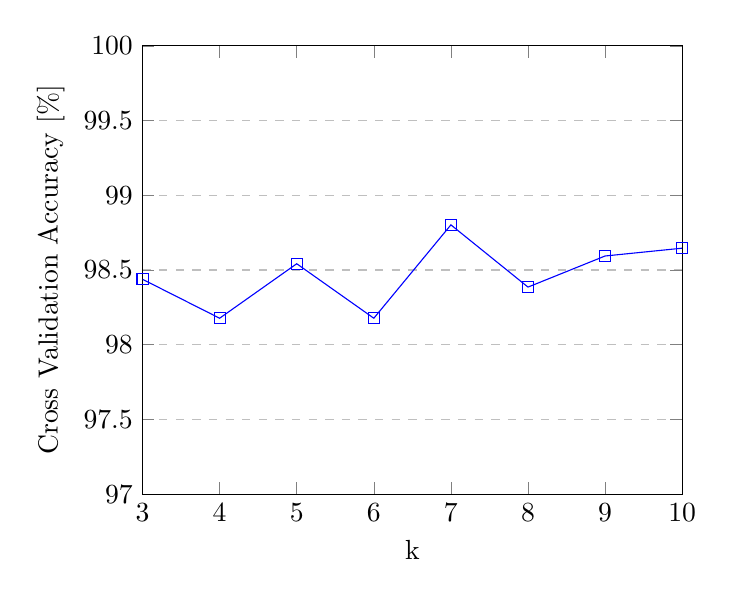
\begin{tikzpicture}
	\begin{axis}[
	xlabel={k},
	ylabel={Cross Validation Accuracy [\%]},
	xmin=3, xmax=10,
	ymin=97, ymax=100,
	xtick={3,4,5,6,7,8,9,10},
	ytick={97.0,97.5,98.0,98.5,99.0,99.5,100},
	ymajorgrids=true,
	grid style=dashed,
	]
	
	\addplot[
	color=blue,
	mark=square,
	]
	coordinates {
		(3,98.4375)(4,98.1771)(5,98.5417)(6,98.1771)(7,98.8018)(8,98.3854)(9,98.5935)(10,98.6458)
	};
	
	\end{axis}
	\end{tikzpicture}
	\caption{The effect of k on k-fold cross validation accuracy.}
	\label{fig:k_fold}
\end{figure}

\bgroup
\def\arraystretch{1.5}
\begin{table}[htbp]
	\caption{5-Fold Cross Validation Accuracy Comparion with Inception}
	\begin{center}
		\begin{tabular}{|l|>{\centering\arraybackslash}m{1.75cm}|>{\centering\arraybackslash}m{1.75cm}|}
			\hline
			& \textbf{Our Classifier} & \textbf{Inception V3} \\
			\hline
			\# \textbf{Accuracy} &  &  \\
			\hline
			\textbf{Runtime} &  &  \\
			\hline
		\end{tabular}
		\label{tab:inception_comp}
	\end{center}
\end{table}
\egroup